\subsection{Known-evidence problems}

The three problems have dimension $D=10$ and vary contour curvature and multimodality while retaining deterministic reference evidences.
They are separate from the fixed JAXNS standard-problem regression suite.
Below $\phi_D(x\mid\mu,\Sigma)$ denotes a $D$-variate normal density.
Figure~\ref{fig:evidence_problems} shows their two-dimensional analogues.

\paragraph{Correlated Gaussian (G10).}
This problem places a shifted, strongly correlated Gaussian likelihood in the tail of an isotropic Gaussian prior,
\begin{align}
    L_{\rm G10}(x)=\phi_{10}(x\mid\mu_{\rm G},\Sigma_\ell),\qquad x\sim\mathcal{N}(0,I).
    \label{eq:g10_likelihood}
\end{align}
Here $\mu_{\rm G}=(3,0,\ldots,0)$, $(\Sigma_\ell)_{ii}=1$, and $(\Sigma_\ell)_{ij}=0.99$ for $i\ne j$.
Gaussian conjugacy gives
\begin{align}
    \log Z_{\rm G10}=\log\phi_{10}(\mu_{\rm G}\mid0,I+\Sigma_\ell)
    =-14.48014927. \label{eq:g10_evidence}
\end{align}
G10 tests compression towards a thin correlated ridge in a unimodal target.

\paragraph{Curved Gaussian (CG10).}
This problem retains the standard normal prior of G10 and bends its likelihood with a volume-preserving shear,
\begin{align}
    L_{\rm CG10}(x)&=\phi_{10}\!\left(T_{0.4}^{-1}(x)\mid\mu_{\rm G},\Sigma_\ell\right),
    \label{eq:cg10_likelihood}\\
    T_\beta(z)&=\left(z_1,z_2+\beta\left[(z_1-3)^2-1\right],z_3,\ldots,z_{10}\right).
\end{align}
The shear is centered on the component's latent first-coordinate mean and variance.
It has unit Jacobian and zero mean displacement of the second coordinate under the latent component.
Conditioning $z_{2:10}$ on $z_1$ reduces the reference evidence to one-dimensional quadrature,
\begin{align}
    \log Z_{\rm CG10}
    =\log\E_{z\sim\mathcal{N}(\mu_{\rm G},\Sigma_\ell)}
       \!\left[\phi_{10}(T_{0.4}(z)\mid0,I)\right]
    =-14.59968329. \label{eq:cg10_evidence}
\end{align}
Adaptive integration and independent 128- and 256-node Gauss--Hermite quadrature agree to better than $10^{-12}$ in log evidence.
CG10 tests the combined effects of compression, strong correlation, and curved contours.

\paragraph{Repository spike--slab mixture (SS10).}\label{sec:ss10}
We use the spike--slab model from the earlier sampler-comparison repository.\footnote{Model source: \url{https://github.com/Joshuaalbert/jaxns-cosmology/blob/67e45dac6d9b273c4f4d957433f53228bf9ea7e0/jaxns_cosmology/models/spikeslab.py}.}
Both components are full ten-dimensional densities; only their first two mean coordinates are shifted.
The prior is uniform on $[-4,8]^{10}$ and
\begin{align}
    L_{\rm SS10}(x)&=\phi_{10}(x\mid\mu_1,0.08I)
                   +\phi_{10}(x\mid\mu_2,0.8I),\label{eq:ss10_likelihood}\\
    \mu_1&=(6,6,0,\ldots,0),\qquad\mu_2=(2.5,2.5,0,\ldots,0).
\end{align}
The covariance diagonals $0.08$ and $0.8$ correspond to standard deviations $\sqrt{0.08}$ and $\sqrt{0.8}$.
Each normalized density has coefficient one; the sum is not divided by two.
At equal component Mahalanobis radius the spike-to-slab geometric volume ratio is $(0.08/0.8)^{10/2}=10^{-5}$; this is not a posterior fraction or a volume ratio at a common likelihood threshold.
Writing $s_1=\sqrt{0.08}$, $s_2=\sqrt{0.8}$ and $\Phi$ for the standard normal cumulative distribution function gives the finite-prior reference
\begin{align}
    Z_{\rm SS10}=12^{-10}\sum_{k=1}^{2}\prod_{j=1}^{10}
    \left[\Phi\!\left(\frac{8-\mu_{kj}}{s_k}\right)
         -\Phi\!\left(\frac{-4-\mu_{kj}}{s_k}\right)\right].\label{eq:ss10_evidence}
\end{align}
Thus $\log Z_{\rm SS10}=-24.15593481$, and the reference spike fraction is $0.5000077444$.
The slab-only log evidence is $-24.84909748$.
SS10 tests recovery of substantial posterior mass in a geometrically small component and provides an ablation of evidence precision when that structure is underrepresented.

\begin{figure*}[t]
    \centering
    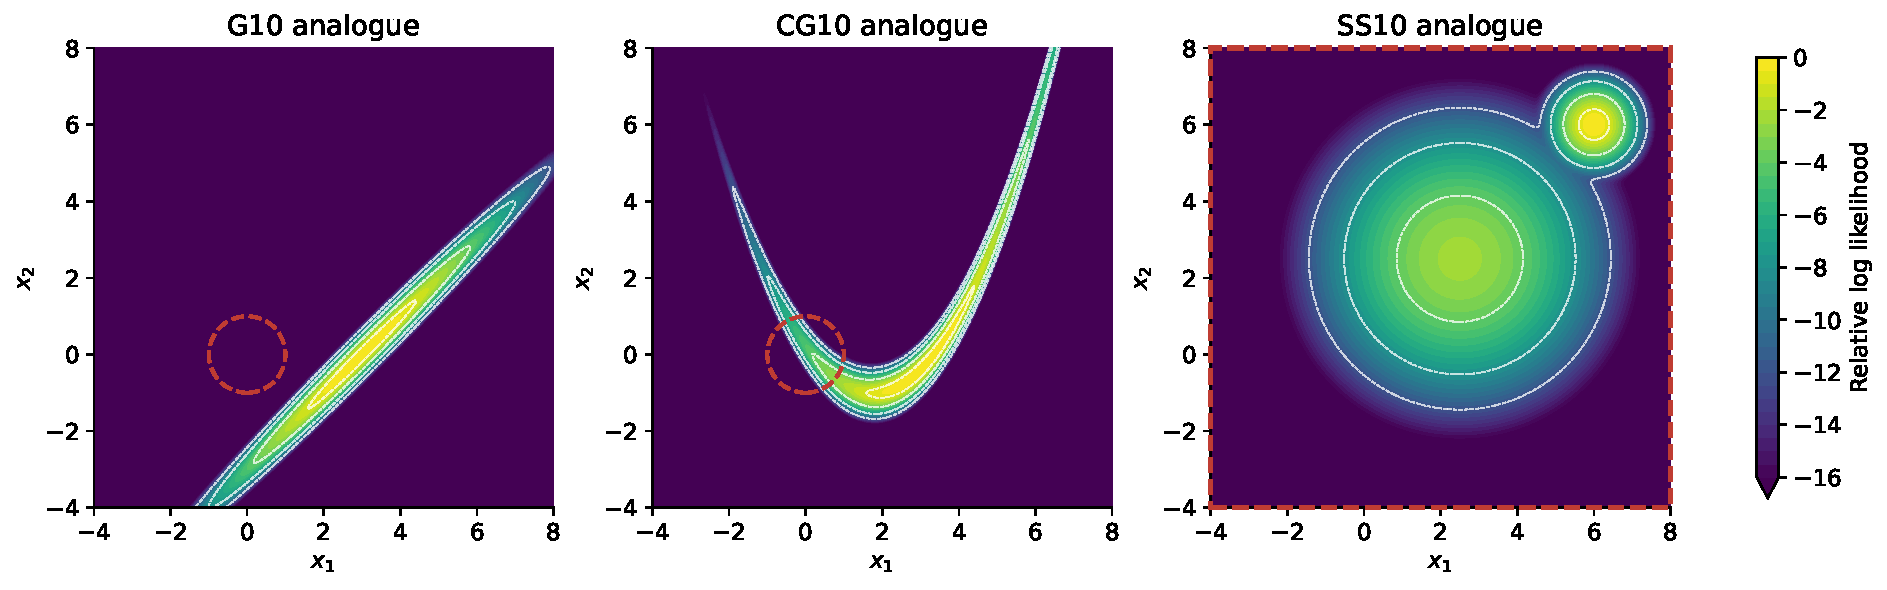
\includegraphics[width=\textwidth]{images/evidence_problems.pdf}
    \caption{Two-dimensional analogues of G10, CG10, and SS10. Filled contours show relative log likelihood; white lines mark selected levels. Red dashed boundaries show the one-$\sigma$ Gaussian prior circle or the support of the uniform prior. These two-dimensional densities are analogues, not posterior marginals of the ten-dimensional problems. The SS10 geometric volume contrast is much larger in ten dimensions than shown here.}
    \label{fig:evidence_problems}
\end{figure*}

\subsection{Paired protocol and metrics}

All evidence tables use A+C with $30$ seeds numbered $0$--$29$ per problem.
The sampler descends from commit \texttt{a18124b}; the frozen experiment source is \texttt{aa79a0d}.
The sparse evidence reducer at \texttt{5667381} handles tied likelihood blocks with the sampler's existing Dirichlet plateau law; its sampler and model source are identical to the frozen run source.
Ties are retained as observed, without jitter or deduplication. For singleton blocks, the revised reducer preserves the original random fields and results exactly.
Intervention A retains every phantom unit-prior coordinate and includes eligible phantom identities in the existing uniform seed-selection rule.
Intervention C uses the evidence-improving allocation target in Appendix~\ref{sec:allocation_targets}.
Each run starts with $d_0=30D=300$ root lineages, completes one uniform discovery goal with \texttt{delta\_K=1}, then adds an evidence-improving allocation gap
\begin{align}
    \Delta K_g=\left\lceil300\,\overline U^Z_g\right\rceil,
\end{align}
where $\overline U^Z$ is normalized to unit peak.
Execution width is $100$; each classic replacement uses $T=10D=100$ isotropic slice transitions without stepping out.
All $99$ intermediate phantom states per chain are retained for seed eligibility.
We condition evidence on their leading prefixes $D,2D,\ldots,9D$, with classic shrinkage denoted $0D$.
Phantom states are not inserted into the posterior sample sequence.

The baseline goal is
\begin{align}
    \widehat\sigma^{\rm exp}_{\log Z}<0.05.\label{eq:benchmark_goal}
\end{align}
The within-goal depth condition is Eq.~\ref{eq:small_remaining_evidence} with $\tau_Z=\log(1+10^{-3})$.
Each tree is reduced with $2048$ paired shrinkage draws per prefix, using prefix increments of $D=10$ and minimum cluster participation count $C_{\min}=20$.
One gamma weight is shared by all retained phantoms from a given chain, including across prefix increments.
The cluster-weight random seeds are controlled across prefixes, and the stopping rule uses classic expected uncertainty throughout.
One CPU is pinned to each worker on dorrie, with at most $60$ concurrent workers; tighter stages reduce concurrency to accommodate their growing phantom storage.

Tables~\ref{tab:phantom_evidence_g10_0p05}--\ref{tab:phantom_evidence_ss10_0p02} report log-evidence bias, RMSE, mean reported shrinkage SD, and empirical coverage of the central $95\%$ shrinkage interval.
Bias errors are across-tree SDs; RMSE errors are bootstrap SEs from $10{,}000$ resamples of the $30$ seeds, with bootstrap seed $20260909$.
Paired bootstrap contrasts use the same resampled trees for classic and phantom RMSE and absolute cohort bias.
For each resample, the latter contrast is $|\overline e_{\rm Ph90}|-|\overline e_{\rm classic}|$, where $e$ is log-evidence error; it is not a difference in mean absolute error.
Bold marks the lowest point-estimate RMSE, not a significance statement.
These intervals quantify shrinkage conditional on the represented tree; they need not cover exploration error.

SS10 spike mass is computed once per classic tree as
\begin{align}
    \widehat m_1=\sum_i w_i^{\rm classic}
       \frac{L_1(x_i)}{L_1(x_i)+L_2(x_i)}.
\end{align}
Using component responsibilities avoids a hard-assignment overlap error.
Every phantom-prefix analysis shares this same classic posterior estimate.

To test whether more sampling recovers the spike, the same $30$ SS10 trees were continued to classic uncertainty $0.02$.
All $30$ continuations and paired reductions completed. Planned further stages at $0.01$ and $0.005$ were cancelled because of computational cost; no completed result at either tighter target is reported.
Before these runs, recovery was defined descriptively as spike-mass RMSE at most $0.05$ with no seed more than $0.15$ from the reference mass.
This criterion governed planned continuation; it is not a formal hypothesis test, and phantom benefit is assessed separately.
Full-capacity checkpoints preserve the stored random streams and buffer layout; trimming is used only for analysis because it changes the subsequent sampling trajectory in this implementation.
Likelihood costs and goal counts for tighter stages are cumulative from the initial tree.
